\documentclass[aspectratio=169,11pt]{beamer}

% Shared style (ib-tutorials.sty at the repo root).
\makeatletter\def\input@path{{./}{../}}\makeatother
\usepackage{ib-tutorials}

\usepackage[utf8]{inputenc}
\usepackage{amsmath,amssymb}
\usepackage{booktabs}
\usepackage{array}
\newcolumntype{L}[1]{>{\raggedright\arraybackslash}p{#1}}
\usepackage{graphicx}
\usepackage{xcolor}
\usepackage{listings}
\usepackage{tikz}
\usetikzlibrary{arrows.meta,positioning,shapes.geometric,fit,calc}
\usepackage{hyperref}

\newcommand{\sourcecredit}[1]{\vfill\hfill{\tiny\textcolor{DarkGray}{#1}}}

\lstset{
  basicstyle=\ttfamily\scriptsize\color{BlackGray},
  keywordstyle=\color{NavyBlue}\bfseries,
  commentstyle=\color{DarkGray}\itshape,
  stringstyle=\color{OliveGreen},
  showstringspaces=false,
  columns=fullflexible,
  keepspaces=true,
  frame=single,
  framerule=0.4pt,
  rulecolor=\color{LightGray},
  backgroundcolor=\color{LightGray!30},
  xleftmargin=0.25em,
  xrightmargin=0.25em
}
\lstdefinestyle{shell}{morecomment=[l]{\#}}
\lstdefinestyle{slurm}{}

\title[Installing IBAMR]{Installing IBAMR with autoibamr}
\subtitle{One script builds IBAMR and every library it needs}
\author[Miller]{Laura A. Miller}
\institute[UArizona]{Department of Mathematics, University of Arizona}
\date{Using IB Software \textbullet\ Part I \textbullet\ Chapter 2}

% the dependency stack, used on the title slide and on slide 4
\newcommand{\stackbox}[3]{\node[draw=DarkGray,rounded corners=1pt,fill=#3,text width=#2,align=center,inner sep=3pt,font=\scriptsize] {#1};}

\begin{document}

% 1
\begin{frame}[plain]
\maketutorialtitlepanel{%
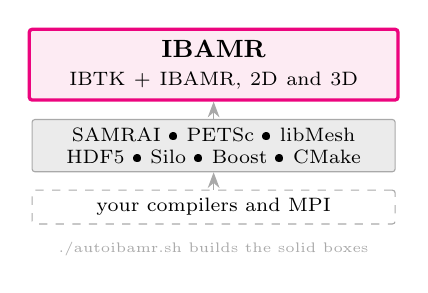
\begin{tikzpicture}[node distance=2.2mm]
  \node[draw=RubineRed,very thick,rounded corners=1pt,fill=RubineRed!8,text width=44mm,align=center,inner sep=4pt,font=\small] (ib) {\textbf{IBAMR}\\[-1pt]{\scriptsize IBTK + IBAMR, 2D and 3D}};
  \node[draw=DarkGray,rounded corners=1pt,fill=LightGray!45,text width=44mm,align=center,inner sep=3pt,font=\scriptsize,below=of ib] (mid) {SAMRAI \textbullet\ PETSc \textbullet\ libMesh\\HDF5 \textbullet\ Silo \textbullet\ Boost \textbullet\ CMake};
  \node[draw=DarkGray,dashed,rounded corners=1pt,text width=44mm,align=center,inner sep=3pt,font=\scriptsize,below=of mid] (sys) {your compilers and MPI};
  \draw[-{Stealth[length=2mm]},DarkGray] (sys) -- (mid);
  \draw[-{Stealth[length=2mm]},DarkGray] (mid) -- (ib);
  \node[font=\tiny,text=DarkGray,below=1mm of sys] {\code{./autoibamr.sh} builds the solid boxes};
\end{tikzpicture}}
\end{frame}

% 2
\begin{frame}{Learning goals}
By the end of this chapter you should be able to:
\begin{enumerate}
  \item say what autoibamr installs and what IBAMR uses each library for;
  \item choose an IBAMR version and a place to install it;
  \item install the prerequisites on Ubuntu, on Windows through WSL2, on macOS, and on Puma;
  \item run autoibamr, follow its progress, and read its log;
  \item load an installation with \code{enable.sh} and test it by building an example;
  \item recognize and fix the most common installation errors.
\end{enumerate}
\vspace{4mm}
\begin{punchbox}
\small Installing IBAMR used to take pages of notes: each library built by hand, with versions that had to match. Those recipes (2011--2019) are kept in Part X, chapter X2. This chapter replaces them.
\end{punchbox}
\end{frame}

% 3
\begin{frame}{What autoibamr is}
\begin{columns}[T,onlytextwidth]
\begin{column}{0.55\textwidth}
\begin{itemize}
  \item A shell script from the IBAMR developers that \al{downloads, configures, builds and installs} IBAMR together with the libraries it needs.
  \item The versions of those libraries are chosen to work with the IBAMR version you ask for.
  \item It runs on Linux and macOS. On Windows it runs inside WSL2, a Linux system that Windows provides.
  \item It is based on \emph{candi}, the installer for the deal.II finite-element library.
  \item It builds IBAMR with CMake, which gives you the \code{IBAMRConfig.cmake} file that application builds look for (chapter 3).
\end{itemize}
\end{column}
\begin{column}{0.42\textwidth}
\begin{block}{Get it}
\small\url{https://github.com/IBAMR/autoibamr}
\end{block}
\begin{block}{IBAMR's own instructions}
\small\url{https://ibamr.github.io/building}
\end{block}
\begin{alertblock}{Why not the old Makefile builds?}
\small Makefile (autotools) builds still work through IBAMR 0.19 but are removed in 0.20. Applications built with Makefiles need a \code{make.inc} file that autoibamr does not create.
\end{alertblock}
\end{column}
\end{columns}
\end{frame}

% 4
\begin{frame}{What gets built, and what each piece does}
\begin{columns}[T,onlytextwidth]
\begin{column}{0.40\textwidth}
\centering
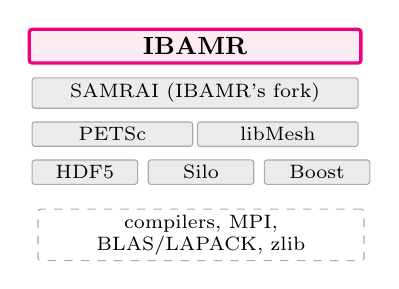
\begin{tikzpicture}[node distance=1.6mm]
  \node[draw=RubineRed,very thick,rounded corners=1pt,fill=RubineRed!8,text width=40mm,align=center,inner sep=3pt,font=\small] (ib) {\textbf{IBAMR}};
  \node[draw=DarkGray,rounded corners=1pt,fill=LightGray!45,text width=40mm,align=center,inner sep=2pt,font=\scriptsize,below=of ib] (sam) {SAMRAI (IBAMR's fork)};
  \node[draw=DarkGray,rounded corners=1pt,fill=LightGray!45,text width=19mm,align=center,inner sep=2pt,font=\scriptsize,below=of sam.south west,anchor=north west] (pet) {PETSc};
  \node[draw=DarkGray,rounded corners=1pt,fill=LightGray!45,text width=19mm,align=center,inner sep=2pt,font=\scriptsize,below=of sam.south east,anchor=north east] (lm) {libMesh};
  \node[draw=DarkGray,rounded corners=1pt,fill=LightGray!45,text width=12mm,align=center,inner sep=2pt,font=\scriptsize,below=of pet.south west,anchor=north west] (h5) {HDF5};
  \node[draw=DarkGray,rounded corners=1pt,fill=LightGray!45,text width=12mm,align=center,inner sep=2pt,font=\scriptsize,right=1.2mm of h5] (silo) {Silo};
  \node[draw=DarkGray,rounded corners=1pt,fill=LightGray!45,text width=12mm,align=center,inner sep=2pt,font=\scriptsize,right=1.2mm of silo] (bo) {Boost};
  \node[draw=DarkGray,dashed,rounded corners=1pt,text width=40mm,align=center,inner sep=2pt,font=\scriptsize,below=3mm of silo] (sys) {compilers, MPI, BLAS/LAPACK, zlib};
\end{tikzpicture}
\end{column}
\begin{column}{0.57\textwidth}
\scriptsize
\begin{tabular}{@{}L{0.22\linewidth}L{0.72\linewidth}@{}}
\toprule
Library & What IBAMR uses it for \\
\midrule
SAMRAI & adaptive Cartesian grids: patches, levels, regridding, parallel data \\
PETSc & vectors, matrices and the Krylov solvers and preconditioners \\
libMesh & finite-element meshes and assembly for IBFE \\
HDF5 & the file format of restart files and of the fluid output in \code{dumps.visit} \\
Silo & the structure (Lagrangian) output in \code{lag\_data.visit} \\
Boost & C++ utilities; bundled with IBAMR until 0.20 \\
CMake & the build system; autoibamr downloads its own copy \\
numdiff & compares numbers in IBAMR's test suite \\
\bottomrule
\end{tabular}
\vspace{3mm}

Versions installed for IBAMR 0.19.0 in October 2026: CMake 3.30.6, HDF5 1.12.2, PETSc 3.23.3, Boost 1.91.0, Silo 4.11, libMesh 1.7.8, SAMRAI 2025.10.29.
\end{column}
\end{columns}
\end{frame}

% 5
\begin{frame}{Which IBAMR version?}
\footnotesize
\begin{tabular}{@{}lllL{0.46\textwidth}@{}}
\toprule
IBAMR & Released & SAMRAI fork & Notes \\
\midrule
0.16.0 & 31 January 2025 & 2025.01.09 & installed on Puma for this course \\
0.17.0 & 1 October 2025 & 2025.09.12 & small fixes \\
0.18.0 & 12 November 2025 & 2025.10.29 & some solver classes take their settings as input databases \\
\al{0.19.0} & 11 March 2026 & 2025.10.29 & \al{autoibamr's default}; velocity is written only as the vector \code{U} \\
0.20 & in development & & CMake builds only; Boost no longer bundled \\
\bottomrule
\end{tabular}
\vspace{5mm}
\begin{itemize}
  \item Every example in this tutorial builds and runs with \textbf{0.16.0 and 0.19.0}.
  \item The one difference you will notice is in VisIt: from 0.19, plot \code{U}, \code{U[0]} or \code{magnitude(U)} instead of \code{U\_x}. Those expressions also work with 0.16.
  \item Starting fresh on a laptop? Take the default, 0.19.0.
  \item The autoibamr help text lists versions up to 0.17.0 only. The script itself installs 0.19.0 by default and accepts \code{--ibamr-version=0.18.0} and \code{0.19.0}.
\end{itemize}
\end{frame}

% 6
\begin{frame}{Where to install it}
\begin{columns}[T,onlytextwidth]
\begin{column}{0.48\textwidth}
\begin{block}{Your own computer}
\begin{itemize}\small
  \item Linux, macOS, or Windows through WSL2.
  \item Good for learning, editing input files, 2D runs and VisIt.
  \item Needs about \textbf{6~GB} of disk: one install with its sources and build files took 5.6~GB.
  \item Builds in about half an hour on a fast laptop with 12 parallel jobs.
\end{itemize}
\end{block}
\end{column}
\begin{column}{0.48\textwidth}
\begin{block}{Puma, the UA cluster}
\begin{itemize}\small
  \item For 3D runs, long runs and parameter sweeps.
  \item \alr{Build inside a job}: the compiler and MPI modules load only on compute nodes, not on the login node.
  \item A class or lab can share one installation in the group's folder, so each student does not spend an hour building.
\end{itemize}
\end{block}
\end{column}
\end{columns}
\vspace{4mm}
\begin{punchbox}
\small You can keep several installs side by side, one per version, with \code{--prefix}. Each has its own \code{enable.sh}; load the one that matches the version an application was built with.
\end{punchbox}
\end{frame}

% 7
\begin{frame}[fragile]{Prerequisites on Ubuntu (and Ubuntu under WSL2)}
autoibamr needs compilers, an MPI library with its compiler wrappers, and a few tools. On Ubuntu 24.04 this one command installs everything; it was used for the tests in this tutorial:
\begin{lstlisting}[style=shell]
sudo apt update
sudo apt install build-essential gfortran openmpi-bin libopenmpi-dev \
    python3 python3-setuptools m4 git wget curl ca-certificates \
    libtirpc-dev zlib1g-dev pkg-config libblas-dev liblapack-dev \
    unzip bzip2 xz-utils patch file
\end{lstlisting}
\begin{columns}[T,onlytextwidth]
\begin{column}{0.52\textwidth}
\begin{itemize}\small
  \item \code{openmpi-bin} and \code{libopenmpi-dev} give \code{mpicc}, \code{mpicxx}, \code{mpif90} and \code{mpirun}.
  \item \code{libtirpc-dev} supplies the XDR functions libMesh needs.
  \item On Ubuntu 22.04, add \code{python3-distutils}.
\end{itemize}
\end{column}
\begin{column}{0.45\textwidth}
Check before you start:
\begin{lstlisting}[style=shell]
mpicc --version
mpirun --version
\end{lstlisting}
\end{column}
\end{columns}
\end{frame}

% 8
\begin{frame}[fragile]{On Windows: install Ubuntu with WSL2}
\begin{enumerate}
  \item Open \textbf{PowerShell as administrator} and run
\begin{lstlisting}[style=shell]
wsl --install -d Ubuntu-24.04
\end{lstlisting}
  Restart if Windows asks, then create a Linux user name and password when Ubuntu starts for the first time.
  \item Open \textbf{Ubuntu 24.04} from the Start menu and follow the Ubuntu steps on the previous slide.
  \item \al{Work in your Linux home folder} (\code{\textasciitilde}), not under \code{/mnt/c}. Windows files are reachable at \code{/mnt/c/Users/<you>}, but reading and writing across that boundary is much slower, which matters for builds and simulation output.
  \item From Windows, your Linux files are at \code{\textbackslash\textbackslash wsl.localhost\textbackslash Ubuntu-24.04\textbackslash home\textbackslash <you>}, so the Windows version of VisIt can open your results directly.
\end{enumerate}
\sourcecredit{Microsoft, ``Install WSL'' (learn.microsoft.com/windows/wsl/install).}
\end{frame}

% 9
\begin{frame}[fragile]{On macOS}
\begin{enumerate}
  \item Install Apple's command-line tools:
\begin{lstlisting}[style=shell]
xcode-select --install
\end{lstlisting}
  \item Install an MPI library with Fortran support, for example Open MPI from Homebrew (\url{https://brew.sh}):
\begin{lstlisting}[style=shell]
brew install open-mpi
\end{lstlisting}
\end{enumerate}
\begin{alertblock}{Known problems on macOS (from the autoibamr README)}
\begin{itemize}\small
  \item Anaconda or Miniconda on your \code{PATH} supplies its own compilers and libraries, which conflict with the build. Remove it from \code{PATH} in the terminal you build in.
  \item Exclude the install folder from Spotlight indexing, in Spotlight's privacy settings.
  \item \code{ld: library not found for -ld\_classic}: update Xcode and its command-line tools.
\end{itemize}
\end{alertblock}
\small These macOS steps were not re-tested for this edition of the tutorial.
\end{frame}

% 10
\begin{frame}[fragile]{On Puma: build inside a batch job}
Clone autoibamr on a login node (see the next slide), then submit this script with \code{sbatch build\_ibamr.slurm}:
\begin{lstlisting}[style=slurm]
#!/bin/bash
#SBATCH --job-name=autoibamr
#SBATCH --account=YOUR_GROUP          # your PI's group name
#SBATCH --partition=standard
#SBATCH --nodes=1
#SBATCH --ntasks=16
#SBATCH --mem-per-cpu=4gb
#SBATCH --time=04:00:00
#SBATCH --output=autoibamr-%j.out

module load gnu13 openmpi5            # the modules the course install uses
export CC=mpicc CXX=mpicxx FC=mpif90
cd ~/autoibamr
./autoibamr.sh --ibamr-version=0.16.0 -j 16 --yes
\end{lstlisting}
\begin{itemize}\small
  \item Leave out \code{--ibamr-version} to get the newest version.
  \item Every job that \emph{uses} IBAMR must load the same two modules (chapter 3).
\end{itemize}
\small This script follows the UA HPC documentation, but it has not yet been run on Puma for this edition of the tutorial.
\end{frame}

% 11
\begin{frame}[fragile]{Get autoibamr and run it}
\begin{lstlisting}[style=shell]
cd ~
git clone https://github.com/IBAMR/autoibamr.git
cd autoibamr
export CC=mpicc CXX=mpicxx FC=mpif90     # the MPI compiler wrappers
./autoibamr.sh -j 8
\end{lstlisting}
\begin{columns}[T,onlytextwidth]
\begin{column}{0.50\textwidth}
\begin{itemize}\small
  \item With no options it installs the newest IBAMR into \code{\textasciitilde/autoibamr}, the folder you cloned.
  \item \al{\code{-j 8}} compiles 8 files at a time. \alr{The default is 1}, which can take many hours.
  \item Pick \code{-j} no larger than your number of cores. As a rule of thumb, allow about 2~GB of memory per job, and lower \code{-j} if memory runs out.
  \item It asks you to confirm before it starts; \code{--yes} answers for you.
\end{itemize}
\end{column}
\begin{column}{0.47\textwidth}
\begin{block}{Common choices}
\scriptsize
\begin{tabular}{@{}ll@{}}
\code{--ibamr-version=0.16.0} & a specific version \\
\code{--prefix=<folder>} & install somewhere else \\
\code{-j 8} or \code{--jobs=8} & parallel compiling \\
\code{--yes} & no questions \\
\end{tabular}
\end{block}
\end{column}
\end{columns}
\end{frame}

% 12
\begin{frame}{More options}
\small
\begin{tabular}{@{}L{0.40\linewidth}L{0.56\linewidth}@{}}
\toprule
Option & What it does \\
\midrule
\code{--enable-debugging} & debug symbols and every assertion checked, no optimization; installs into \code{\textasciitilde/autoibamr-debug}. Use it to track down a crash, not for production runs. \\
\code{--enable-assertions-}\newline\code{\ \ with-optimizations} & assertions with optimization: catches many mistakes for a 10--20\% slowdown \\
\code{--enable-native-optimizations} & tunes the code for the processor it is built on. Use only when you build on the same kind of machine you run on. \\
\code{--dependencies-only} & everything except IBAMR itself \\
\code{--disable-libmesh} & no libMesh, so no IBFE \\
\code{--external-boost=<path>} & use a Boost you already have \\
\code{--lapack-library=fblaslapack} & a slower but simpler LAPACK than the default OpenBLAS, useful with profiling tools \\
\code{--enable-exodusii} & also builds NetCDF and ExodusII, which some other packages need \\
\bottomrule
\end{tabular}
\vspace{2mm}

Run \code{./autoibamr.sh --help} for the full list.
\end{frame}

% 13
\begin{frame}[fragile]{How long it takes}
The end of the screen output from the two installs made for this tutorial (a 24-core laptop running Ubuntu 24.04 under WSL2, 12 parallel jobs):
\begin{columns}[T,onlytextwidth]
\begin{column}{0.48\textwidth}
\begin{lstlisting}
IBAMR 0.16.0
Build finished in 1477 seconds.
Summary of timings:
cmake: 7 s
hdf5: 136 s
petsc: 240 s
boost: 54 s
numdiff: 10 s
silo: 22 s
libmesh: 174 s
samrai: 52 s
ibamr: 779 s
\end{lstlisting}
\end{column}
\begin{column}{0.48\textwidth}
\begin{lstlisting}
IBAMR 0.19.0
Build finished in 1730 seconds.
Summary of timings:
cmake: 6 s
hdf5: 121 s
petsc: 253 s
boost: 71 s
numdiff: 10 s
silo: 25 s
libmesh: 187 s
samrai: 63 s
ibamr: 993 s
\end{lstlisting}
\end{column}
\end{columns}
\begin{itemize}\small
  \item About half an hour each. IBAMR itself is more than half of the time.
  \item With 4 parallel jobs, expect roughly three times as long.
\end{itemize}
\end{frame}

% 14
\begin{frame}[fragile]{What is in the install folder}
\begin{lstlisting}
~/autoibamr/
  autoibamr.sh  autoibamr.log      the script and its log
  configuration/
    enable.sh                      source this to use the install
    IBAMR-0.19.0  petsc-3.23.3 ... one small settings file per package
  packages/
    IBAMR-0.19.0/                  include/, lib/, lib/cmake/ibamr/IBAMRConfig.cmake
    petsc-3.23.3/  libmesh-1.7.8/  samrai-2025.10.29/  silo-4.11-bsd/ ...
    cmake-3.30.6/                  autoibamr's own copy of CMake
  tmp/
    src/                           downloaded source archives
    unpack/IBAMR-0.19.0/           IBAMR's source, including examples/
    build/v0.19.0/                 IBAMR's build folder, used to build the examples
\end{lstlisting}
\begin{punchbox}
\small \code{autoibamr.log} is written in the folder you ran the script from. If a build fails, search it for the \emph{first} error; later errors usually follow from it.
\end{punchbox}
\end{frame}

% 15
\begin{frame}[fragile]{Using the install: \code{enable.sh}}
Each new terminal, and each batch job, starts by loading the install:
\begin{lstlisting}[style=shell]
source ~/autoibamr/configuration/enable.sh
\end{lstlisting}
It runs the small settings files in \code{configuration/}. For example, it sets these (with the full path of your home folder):
\begin{lstlisting}[style=shell]
export IBAMR_ROOT=~/autoibamr/packages/IBAMR-0.19.0
export PETSC_DIR=~/autoibamr/packages/petsc-3.23.3
export PATH=~/autoibamr/packages/cmake-3.30.6/bin:${PATH}
\end{lstlisting}
\begin{itemize}\small
  \item \code{IBAMR\_ROOT} is how CMake finds IBAMR when you build an application (chapter 3).
  \item \code{cmake} now means autoibamr's copy, which is new enough for IBAMR.
  \item To load it automatically, add the \code{source} line to \code{\textasciitilde/.bashrc}. If you keep two versions, load each by hand instead.
  \item On Puma, load the modules first: \code{module load gnu13 openmpi5}.
\end{itemize}
\end{frame}

% 16
\begin{frame}[fragile]{Test the install with an upstream example}
IBAMR's own examples build inside the install's build folder:
\begin{lstlisting}[style=shell]
source ~/autoibamr/configuration/enable.sh
cd ~/autoibamr/tmp/build/v0.19.0
make -j 4 IB-ex1                     # about half a minute
cd examples/IB/explicit/ex1
mpirun -np 4 ./main2d input2d
\end{lstlisting}
\begin{itemize}\small
  \item \code{IB-ex1} is an elastic membrane, the upstream relative of this tutorial's rubber band (example IB/01).
  \item Its input files are copied next to \code{main2d}, so it runs from that folder.
  \item \code{make examples-IB} builds every IB example. Chapter 15 tours them.
\end{itemize}
\begin{punchbox}
\small If this example builds and runs, the installation works. Chapter 3 builds your own programs outside this folder.
\end{punchbox}
\end{frame}

% 17
\begin{frame}{When something goes wrong}
\scriptsize
\begin{tabular}{@{}L{0.45\linewidth}L{0.51\linewidth}@{}}
\toprule
What you see & What to do \\
\midrule
\code{CC variable not set. Please set it with \$export CC=<(MPI) C compiler>} & \code{export CC=mpicc CXX=mpicxx FC=mpif90}, then run again \\
\code{c++: fatal error: Killed signal terminated program cc1plus} & the computer ran out of memory: lower \code{-j} \\
libMesh cannot find XDR or \code{rpc/rpc.h} & install \code{libtirpc-dev} (Ubuntu) \\
\code{mpirun has detected an attempt to run as root} & build and run as your own user, not with \code{sudo} \\
\code{ld: library not found for -ld\_classic} on macOS & update Xcode and its command-line tools \\
errors that mention \code{anaconda} or \code{miniconda} paths & remove Anaconda from \code{PATH} in this terminal \\
on Puma, \code{module: command not found} or modules missing & you are on a login node: build inside a batch job \\
\bottomrule
\end{tabular}
\vspace{3mm}

\small For anything else, find the first error in \code{autoibamr.log} and ask on the IBAMR discussion forum: \url{https://github.com/IBAMR/IBAMR/discussions}.
\end{frame}

% 18
\begin{frame}{Summary}
\begin{enumerate}
  \item autoibamr builds IBAMR and matching versions of SAMRAI, PETSc, libMesh, HDF5, Silo and Boost in one command.
  \item Install the prerequisites first: compilers, MPI with \code{mpicc}/\code{mpicxx}/\code{mpif90}, and a few tools.
  \item Run \code{./autoibamr.sh -j N}. Always give \code{-j}; add \code{--ibamr-version} for an older version.
  \item On Puma, build inside a batch job after \code{module load gnu13 openmpi5}.
  \item Load an install with \code{source \ldots/configuration/enable.sh}, which sets \code{IBAMR\_ROOT}.
  \item Test it by building \code{IB-ex1} in \code{tmp/build/v<version>}.
\end{enumerate}
\vspace{3mm}
\begin{homebox}
\small Next, chapter 3: build and run your own IBAMR program with CMake, starting with the rubber band.
\end{homebox}
\end{frame}

% 19
\begin{frame}{References}
\small
\begin{itemize}
  \item IBAMR developers. \emph{autoibamr}. \url{https://github.com/IBAMR/autoibamr} (commit \code{9c1e0a5}, October 2026).
  \item IBAMR developers. \emph{Building IBAMR}. \url{https://ibamr.github.io/building}.
  \item IBAMR developers. \emph{Building IBAMR applications}. \url{https://ibamr.github.io/applications}.
  \item deal.II developers. \emph{candi: compile and install}. \url{https://github.com/dealii/candi}.
  \item Microsoft. \emph{Install WSL}. \url{https://learn.microsoft.com/windows/wsl/install}.
  \item The tests in this chapter used Ubuntu 24.04.5 under WSL2 with GCC 13.3.0 and Open MPI 4.1.6.
\end{itemize}
\end{frame}

\end{document}
